%%%%%%%%%%%%%%%%%%%%%%%%%%%%%%%%%%%%%%%%%%%%%%%%%%%%%%%%%%%%%%%%%%%%%%%
% Sample template for MIT Junior Lab Student Written Summaries
% Available from http://web.mit.edu/8.13/samplepaper/sample-paper.tex
%
% Last Updated June 20, 2004
%
% Adapted from the American Physical Societies REVTeK-4 Pages
% at http://publish.aps.org
%
% ADVICE TO STUDENTS: Each time you write a paper, start with this
%    template and save under a new filename.  If convenient, don't
%    erase unneeded lines, just comment them out.  Often, they
%    will be useful containers for information.
%%%%%%%%%%%%%%%%%%%%%%%%%%%%%%%%%%%%%%%%%%%%%%%%%%%%%%%%%%%%%%%%%%%%%%%


%%%%%%%%%%%%%%%%%%%%%%%%%%%%%%%%%%%%%%%%%%%%%%%%%%%%%%%%%%%%%%%%%%%%%%%
% PREAMBLE
% The preamble of a LaTeX document is the set of commands that precede
% the \begin{document} line.  It contains a \documentclass line
% to load the REVTeK-4 macro definitions and various \usepackage
% lines to load other macro packages.
%
% ADVICE TO STUDENTS: This preamble contains a suggested set of
%     class options to generate a ``Junior Lab'' look and feel that
%     facilitate quick review and feedback from one's peers, TA's
%     and section instructors.  Don't make substantial changes without
%     first consulting your section instructor.
%%%%%%%%%%%%%%%%%%%%%%%%%%%%%%%%%%%%%%%%%%%%%%%%%%%%%%%%%%%%%%%%%%%%%%%

\documentclass[aps,twocolumn,secnumarabic,nobalancelastpage,amsmath,amssymb,nofootinbib]{revtex4}

% nofootinbib is another document class option that allows you to put
% footnotes on the page where they occur rather than at the end of the
% paper.  This makes for easier reading!

% secnumarabic is a particularly nice way of identifying sections by
% number to aid electronic review and commentary.

% amsmath and amssymb are necessary for the subequations environment
% among others

\usepackage{graphics}        % standard graphics specifications
\usepackage{graphicx}        % alternative graphics specifications
\usepackage{longtable}       % helps with long table options
\usepackage{url}             % for on-line citations
\usepackage{bm}              % special 'bold-math' package
\usepackage[usenames]{color} %used for font color
\usepackage[utf8]{inputenc}  %useful to type directly diacritic characters
\usepackage{blindtext}
\usepackage{enumitem}
\usepackage{alltt}
\usepackage{nicefrac}
\usepackage{mathtools}
\RequirePackage{bm,xparse,physics}

\begin{document}
\title{Catheter DT20190930}
\author         {John J. Lee}
\email          {jjlee@wustl.edu}
\homepage       {https://wustl.edu}
\affiliation    {Mallinckrodt Institute of Radiology, Washington University, Saint Louis, MO}
\date{\today}

\begin{abstract}
This document describes models for describing the arterial input function
(AIF) in vivo.  
\end{abstract}

\maketitle

%%%%%%%%%%%%%%%%%%%%%%%%%%%%%%%%%%%%%%%%%%%%%%%%%%%%%%%%%%%%%%%%%%%%%%%%%%%%%
\section{Introduction}

The arterial input function (AIF) provides the boundary conditions 
for tracer kinetic problems.  The boundaries are Gaussian surfaces
across which tracers migrate by fluid mechanics and satisfy continuity
equations.  In general, the AIF cannot be directly measured for arbitrary 
volumes such as anatomical structures in vivo.  The most common direct 
measurement obtains from cannulation and automated sampling of the radial 
artery.  The cannulating catheters introduce additional delays and 
dispersions which require correction.  There are also delays and dispersion
that are discrepant between the AIF measured at the radial artery and AIFs
which describe the internal carotid artery, basilar artery or distal
arterioles.  Consequently, a model of the AIF is always necessary.  The
classes *Catheter* in this package provide such models.  

All source codes, testing codes, documentation and ancillary data are
available at \url{https://github.com/jjleewustledu/mlswisstrace}.  
All Matlab codes are packaged as $\texttt{mlswisstrace}$ unless
indicated otherwise.




%%%%%%%%%%%%%%%%%%%%%%%%%%%%%%%%%%%%%%%%%%%%%%%%%%%%%%%%%%%%%%%%%%%%%%%%%%%%%
\section{Guidelines for Good Writing \cite{pritchard1990}}

The essence of expository writing is the communication of
understanding through a clear and concise presentation of
predominately factual material. Most people cannot compose
successful expository prose unless they put the need to communicate
foremost among their priorities. Two things predominate in
generating understanding in the reader:
\begin{enumerate}
\item ORGANIZATION: The reader must be provided with an overview or
outline, know how each fact that he reads fits into that overall
picture, and he must be alerted if it is an especially important
fact. Furthermore, the facts must be presented in a logical order
(so that fact 17 is not important for understanding fact 12).

\item UNIFORM DEPTH of PRESENTATION: Bearing in mind the preexisting
knowledge of the reader, the writer must budget the length of
discussion allotted to each topic in proportion to its importance.

\end{enumerate}

Of course clarity of presentation and elegance of explanation will
greatly enhance the ease and pleasure of understanding; still, a
murky explanation can be fairly useful if the reader has been told
what he is reading about and where it fits into the overall scheme
of things - especially if the reader is familiar with the general
subject matter under discussion.

The Junior lab writeup is one of the few opportunities
undergraduates are given to practice technical writing. Thus we urge
you to concentrate on your overall presentation, not only on the
facts themselves. We strongly recommend that you:
\begin{enumerate}
\item Base your report on an outline.
\item Begin each paragraph with a topic sentence which expresses the
main area of concern and the main conclusion of the paragraph. Put
less important material later in the paragraph.
\end{enumerate}

Point 2 is frequently absent in 8.13 reports; they are your
mechanism for telling the reader what the topic under discussion is
and where it fits into the overall picture.

You can check your topic sentences by reading them in order (i.e.
omit all the following sentences in each paragraph) - this should
give a fair synopsis of your paper.

If you are individually writing up results you obtained with a
partner, use we and I appropriately.

Use the past tense for your procedure and analysis, the past perfect
for preparation and the present for emphasis or conclusions, e.g.
Since we had previously installed Matlab, we quickly concluded that
electrons are waves.

\begin{enumerate}
\item Be sure your Figures have comprehensible captions.

\item Make a complete estimate of your errors (not just statistical) - even
if it's crude.

\item Trace origin of formulae you use (eg. Moseley's Law) to well known
physics (in this case to the Bohr atom) - don't derive, just
indicate what new assumptions are needed.
\end{enumerate}

Please consult the MIT's Online Writing and Communications
Center's web page at \url{http://web.mit.edu/writing/} for further
guidance in all aspects of writing, style and to make appointments
with consultants for free advice.  



%%%%%%%%%%%%%%%%%%%%%%%%%%%%%%%%%%%%%%%%%%%%%%%%%%%%%%%%%%%%%%%%%%%%%%%%%%%%5

\section{Theory}

The report should be type-written in a form that would be suitable
for submission as a manuscript for publication in a professional
journal such as the American Journal of Physics - Physical Review
Letters, \url{http://prl.aps.org/}.  One helpful website is the APS
Physics Review Style and Notation Guide at
\url{http://publish.aps.org/STYLE/}.  Figures (created as PDF files)
should be inserted into the text in their natural positions. The
body of the summary should include a discussion of the theoretical
issues addressed by the experiment.  This should be done at a level,
so that another 8.13 student could follow your development.

\subsection{Typesetting Mathematics}

One of the great powers of \LaTeX is it's ability to typeset all
manner of mathematical expressions.  While it does take a short
while to get used to the syntax, it will soon become second nature.
Numbered, single-line equations are the most common type of equation
in \textit{Junior Lab papers} and are usually referenced in the
text; e.g. see Equation~(\ref{eq:first-equation}).
%
\begin{equation}
   \chi_+(p)\alt{\bf [}2|{\bf p}|(|{\bf p}|+p_z){\bf ]}^{-1/2}
   \left(
   \begin{array}{c}
      |{\bf p}|+p_z\\
      px+ip_y
   \end{array}\right)
\,. \label{eq:first-equation}
\end{equation}
%
% Be sure there is NO EMPTY LINE after \end{quation} and before the
% following lines, if you do not want a new paragraph to start there
% (and be indented).
%
Mathematics can also be placed directly in the text using
delimeters: $\vec{\psi_1} = |\psi_1\rangle \equiv c_0|0\rangle +
c_1|1\rangle \chi^2 \approx
\prod\sum\left[\frac{y_i-f(x_i)}{\sigma_i}\right]^2 |\psi_1\rangle
\sim \lim_{\mu \rightarrow \infty}p(x;\mu) \geq \frac{1}{\sqrt{2 \pi
\mu}} e^{-(x-\mu)^2 / 2\mu}P(x) \ll \int_{-\infty}^x p(x')dx'a
\times b \pm c \Rightarrow \nabla \hbar$.

Infrequently, you may wish to typeset long equations which span more
than one line of a two-column page.  A good solution is to split-up
the equation into multiple lines and label all with a single
equation number, like in Equation~\ref{eq:multilineeq}.  See the
\LaTeX file to see how this is done.
%
\begin{eqnarray}
  \sum \vert M^{\text{viol}}_g \vert ^2
   &=&  g^{2n-4}_S(Q^2)~N^{n-2} (N^2-1)
\nonumber
\\
   &&   \times \left( \sum_{i<j}\right) \sum_{\text{perm}}
            \frac{1}{S_{12}}  \frac{1}{S_{12}} \sum_\tau c^f_\tau
\,.
\label{eq:multilineeq}
\end{eqnarray}

Finally, it is often useful to group related equations to denote their
relationship, e.g. in a derivation.  Enclosing single-line and
multiline equations in \verb+\begin{subequations}+ and
\verb+\end{subequations}+ will produce a set of equations that are
``numbered'' with letters, as shown in Equations.~(\ref{subeq:1}) and
(\ref{subeq:2}) below:
\begin{subequations}
\label{eq:whole}
\begin{equation}
  \left\{
      abc123456abcdef\alpha\beta\gamma\delta1234556\alpha\beta
       \frac{1\sum^{a}_{b}}{A^2}
  \right\}
%
\,\label{subeq:1}
\end{equation}
\begin{eqnarray}
  {\cal M} &=& ig_Z^2(4E_1E_2)^{1/2}(l_i^2)^{-1}
                (g_{\sigma_2}^e)^2\chi_{-\sigma_2}(p_2)
\nonumber\\
  &&\times [\epsilon_i]_{\sigma_1}\chi_{\sigma_1}(p_1).\label{subeq:2}
\end{eqnarray}
\end{subequations}


%%%%%%%%%%%%%%%%%%%%%%%%%%%%%%%%%%%%%%%%%%%%%%%%%%%%%%%%%%%%%%%%%%%%%%%%%%%%%
\section{Materials and Methods}

Function $\texttt{calibrateCatheter2}$ from class 
$\texttt{TwiliteCatheterCalibration}$ describes how tabulated measurements, 
including bench-top hematocrit measurements, were passed to class 
$\texttt{CatheterModel2}$ to estimate dispersion and delay characteristics 
of the catheter apparatus.  

The phantom is shown in Figure~\ref{fig:catheter-phantom}.  The catheter
assembly is schematically described in Figure~\ref{fig:photo-schematic}.  
Impulse-response trials comprised switching the inflow needle from the 
unlabelled reservoir to the $^{18}$FDG-labelled reservoir with the most
rapid possible manual switching so that the labelled impulse lasted 120.0 
seconds.  The impulse duration was much shorter than the half-life of
$^{18}$FDG and no attempt was made to adjust for tracer radiodecay.

\begin{figure}[h]
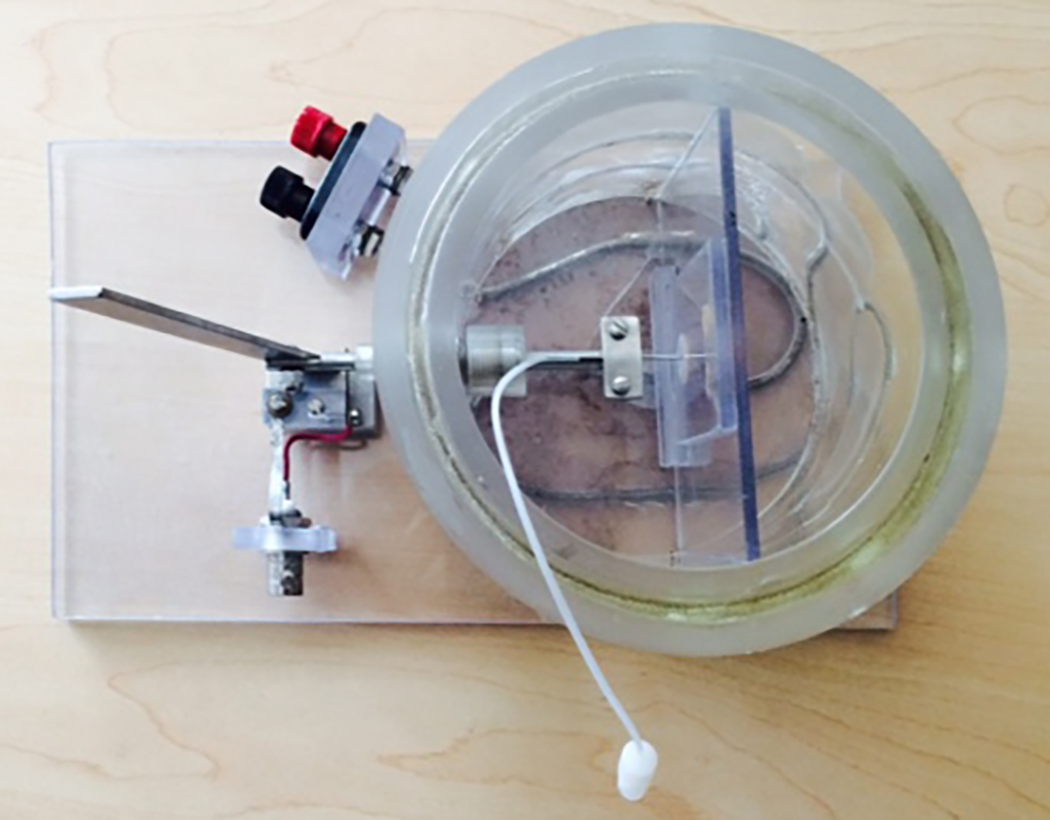
\includegraphics[width=8cm]{catheter-phantom.png}
\caption{Phantom courtesy of Abraham Z. Snyder.  Following assembly with proximal extensions and valves, the estimated volume from blood supply to the edge of the Twilite detection zone was 1.50 mL.\label{fig:catheter-phantom}}
\end{figure}

\begin{figure}[h]
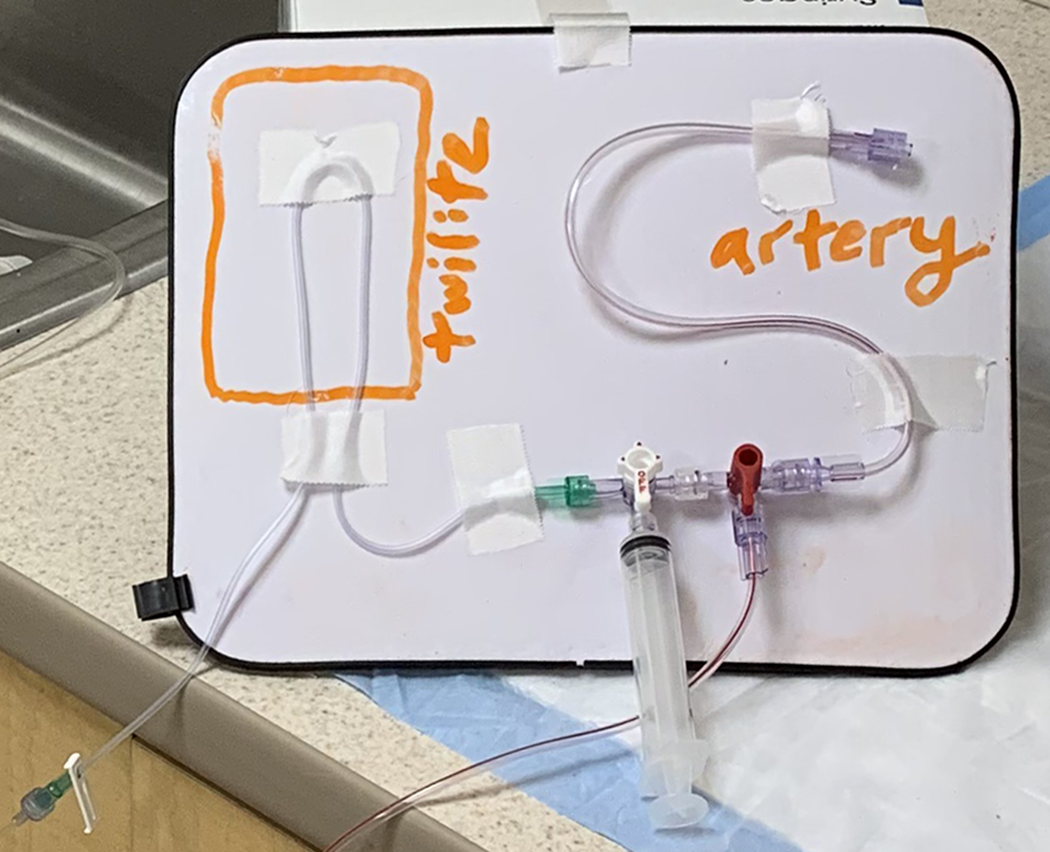
\includegraphics[width=8cm]{photo-schematic.png}
\caption{The proximal extension and valves with 1.348 ml interior volume were packaged as pressure monitoring set REF C-PMS-2502-15-3.5 and REF G07943 (Cook Inc., Bloomington, IN).  The microbore extension set had priming volume 0.642 mL and was packaged as REF V5424 (B. Braun Medical Inc., Bethlehem, PA).  The Twilite probehead enclosed ~20 cm (0.3 mL) of the microbore extension distal to 3 cm (0.04 mL) of tubing slack. \label{fig:photo-schematic}}
\end{figure}

%%%%%%%%%%%%%%%%%%%%%%%%%%%%%%%%%%%%%%%%%%%%%%%%%%%%%%%%%%%%%%%%%%%%%%%%%%%%%
\section{Data and Results}

The final model comprised a generalized gamma distribution with polynomial
adjustment and additional linear adjustments for fractional hematocrit:
%
\begin{align}
	K(t) &\sim \qty(t - t_0)^\alpha e^{-\beta\qty(t - t_0)^p} 
	           \qty[1 + \frac{w \qty(t - t_0)}{1 + w t_0}] \\
	\alpha &= 0.72507 \, \text{Hct} - 0.13201 \\
	\beta &= 0.59645 \, \text{Hct} + 0.69005 \\
    p &= -0.14628 \, \text{Hct} + 0.58306 \\
	w &= 0.040413 \, \text{Hct} + 1.2229 \\
	t_0 & = 9.87 \\
	K(t) &\coloneqq \frac{K(t)}{\int dt' K(t')}
\end{align}
%
with $K(t) := 0$ for $t < t_0$.

All papers should have at least one graphic showing some assemblage of
raw data, see for example Figure~\ref{fig:panel2x2}. There should also
be one graphic which summarizes the experimental data, and which
conveys primary finding(s) of the laboratory exercise.  You may find
that you need more but these two should be a minimum.  Finally, it can
be useful in some circumstances to have a table of results, see
Table~\ref{tab:table1}

\begin{figure*}[htb]
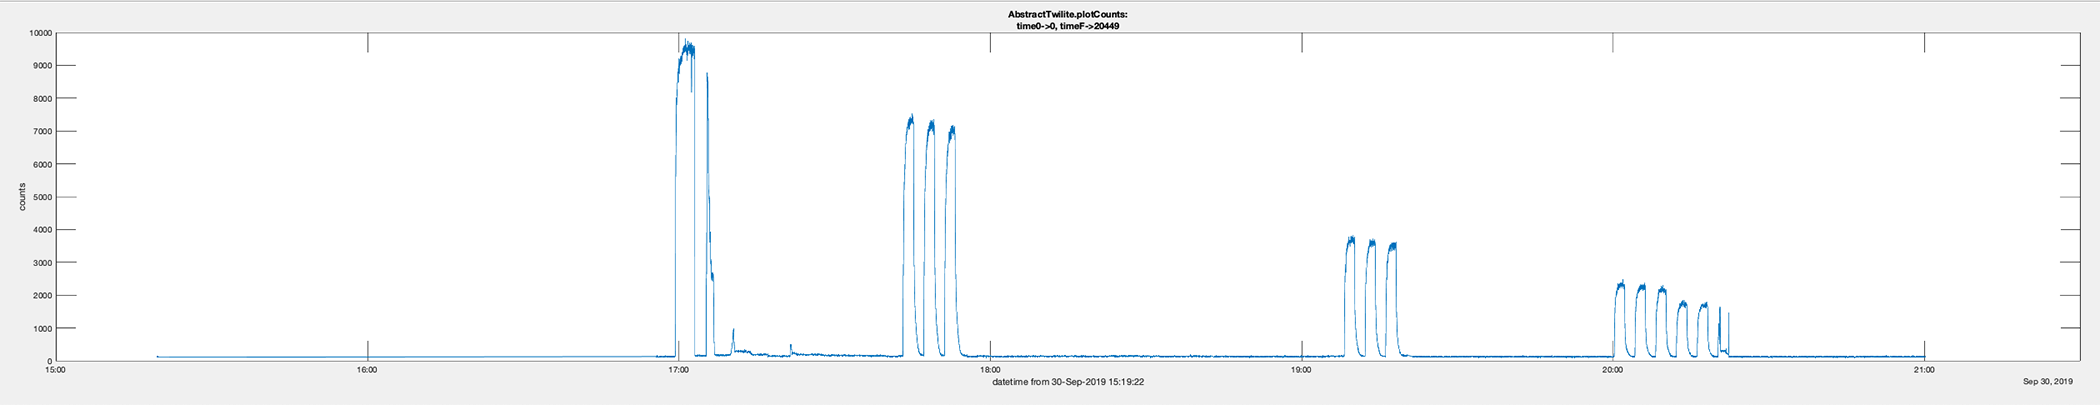
\includegraphics[angle=90,width=4.5cm]{twilite-catheter-calibration-20190930.png}
\caption{Figures can be
rotated using the angle command, see the TeX file for details.  If a
figure is to be placed after the main text use the ``figure*'' option
to make it extend over two columns, see the \LaTeX file for how this
was done.}
\label{fig:twilite}
\end{figure*}

\begin{figure*}[htb]
\includegraphics[angle=0,width=17cm]{TwiliteCatheterCalibration}
\caption{Left panel shows emissions, model fit and best parameters.  Right panel
shows the covariance of distributions.  Similar results were obtained for each of the 
trials of impulse-response.}
\label{fig:twiliteCC_LRw}
\end{figure*}

Try to avoid the temptation to inundate the reader with too many
graphics.  It is worth spending some time thinking of how best to
present information rather than just creating graph after graph of
uninformative data.  All figures and tables must be properly
captioned.  Material and ideas drawn from the work of others must be
properly cited, and a list of references should be included at the end
of the text but before the graphics.

\begin{table}[h]
\caption{\label{tab:table1}A example table with footnotes.  Note that several entries share the same
footnote. Inspect the \LaTeX\ input for this table to see
exactly how it is done.}
\begin{ruledtabular}
\begin{tabular}{cccccccc}
 &$r_c$ (\AA)&$r_0$ (\AA)&$\kappa r_0$&
 &$r_c$ (\AA) &$r_0$ (\AA)&$\kappa r_0$\\
\hline
Cu& 0.800 & 14.10 & 2.550 &Sn\footnotemark[1] & 0.680 & 1.870 & 3.700 \\
Ag& 0.990 & 15.90 & 2.710 &Pb\footnotemark[1] & 0.450 & 1.930 & 3.760 \\
Tl& 0.480 & 18.90 & 3.550 & & & & \\
\end{tabular}
\end{ruledtabular}
\footnotetext[1]{Here's the first, from Ref.~\cite{bevington2003}.}
\end{table}




%%%%%%%%%%%%%%%%%%%%%%%%%%%%%%%%%%%%%%%%%%%%%%%%%%%%%%%%%%%%%%%%%%%%%%%%%%%%%
\section{Conclusions}

And finally, conclusions.  Remember to report all your results with
appropriate significant digits, units, and uncertainties, e.g. Q =
(2.12 $\pm$ 0.06) disintegrations s$^{-1}$.  It is often very useful
to express the quality of your result by measuring how many standard
deviations it lies from other published values.




%%%%%%%%%%%%%%%%%%%%%%%%%%%%%%%%%%%%%%%%%%%%%%%%%%%%%%%%%%%%%%%%%%%%%%%%%%%%%
\section{The Bibliography}
Bibliographic entries may be made either in the `.tex' file itself or within a
separate `.bib' file which gets attached during process of building a
final PDF document.  This latter method is the preferred method and is
then one used in this template by default.  An example of the
alternative style, currently commented out,  is contained in the `.tex' source file.

%%%%%%%%%%%%%%%%%%%%%%%%%%%%%%%%%%%%%%%%%%%%%%%%%%%%%%%%%%%%%%%%%%%%%%%%%%%%%
% Place all of the references you used to write this paper in a file
% with the same name as following the \bibliography command
%%%%%%%%%%%%%%%%%%%%%%%%%%%%%%%%%%%%%%%%%%%%%%%%%%%%%%%%%%%%%%%%%%%%%%%%%%%%%

\bibliography{sample}

%\bibliographystyle{prsty}
%\begin{thebibliography}{99}
%\bibitem{melissinos1966}Melissinos, A.C., Experiments in Modern
%  Physics - 1st Edition, Academic Press,  [1966]
%\bibitem{melissinos2003}Melissinos, A.C., Napolitano, J.,  Experiments in Modern
%  Physics - 2nd Edition, Academic Press,  [2003]
%\bibitem{bevington2003}Bevington and Robinson, Data Reduction and
%  Error Analysis for the Physical Sciences - 3rd Edition, McGraw-Hill,
%  [2003]
%\bibitem{pritchard1990}Professor D. Pritchard, Personal Communication
%\end{thebibliography}


%%%%%%%%%%%%%%%%%%%%%%%%%%%%%%%%%%%%%%%%%%%%%%%%%%%%%%%%%%%%%%%%%%%%%%%%%%%%%
\begin{acknowledgments} FAC gratefully acknowledges Dr. Francine Brown for
her early reviews of this manuscript.
\end{acknowledgments}

%%%%%%%%%%%%%%%%%%%%%%%%%%%%%%%%%%%%%%%%%%%%%%%%%%%%%%%%%%%%%%%%%%%%%%%%%%%%%
\clearpage
\appendix



\section{Using \LaTeX~ Under Windows}
For those students who would like to use a Windows platform, MiKTeX
(pronounced \emph{mik-tech} is a freely available, implementation of
TeX and related programs available from \url{www.miktex.org}. Note
that MiKTeX itself runs from a command line prompt and is not terribly
convenient.  We strongly recommend you simultaneously purchase and
install a very nice TeX editor/shell called WinEdt, available from
\url{www.winedt.com} for only \$30 for students. This interface is
substantially easier than using `emacs' on Athena for writing and
typesetting scientific papers and we encourage you to check it out.

Once you've installed the above software, you will need to obtain the
group of files listed in the next section and put them on your Windows
machine in order to `rebuild' this document from scratch.  MIT offers
free of charge to students (\url{http://web.mit.edu/software/win.html}
a variety of useful software for communicating between your Windows
machine and your Athena account.  Three packages you should obtain and
install are:
\begin{verbatim}
SecureFX
SecureCRT
X-Win32
\end{verbatim}

If you wish to view postscript files under Windows, we
suggest downloading and installing Ghostscript available from
\url{www.cs.wisc.edu/~ghost}.





\section{Using \LaTeX~ Under Athena}
For students wishing to utilize MIT's Athena environment, it is also
a simple process to create your documents.  You can use the following
commands verbatim or tweak them to suit your own organizational system.

In your home directory on Athena, create a convenient directory structure for all of your Junior Lab
work. Type:
\begin{verbatim}
> mkdir ~/8.13
> mkdir ~/8.13/papers
> mkdir ~/8.13/papers/template
> cd ~/8.13/papers/template
\end{verbatim}
Once this (or similiar) directory structure has been created, copy all
of the files needed to compile the template from the Junior Lab locker
into your own Athena account: Type: 
\begin{verbatim}
> setup 8.13
> cp /mit/8.13/www/Samplepaper/* .  
\end{verbatim}
The final period above places the
copied files into the current directory so make sure you're in the
correct directory!  You can see where you are by typing:
\begin{verbatim}
> pwd
\end{verbatim}
The following files should now be in
your current directory: 
\begin{verbatim}
sample-paper.tex
sample-paper.bib
sample-fig1.pdf 
sample-fig3.pdf 
typical-fit-plot.pdf
\end{verbatim}
Additional files may also have been copied but don't worry, these get
regenerated when you build your PDF document.

The `setup' command automatically
appends to your path the location of the {\bf RevTeX-4} files.

Now let's build the file (omitting the `.tex' suffix in the following steps).  

%First type: {\tt > add ghostscript}.  The
%final step in the `build' file uses the ps2pdfwr utility to convert a
%POSTSCRIPT version of your paper into a more easily viewed PDF format.
%This utility is in the `ghostscript' locker on Athena.  


\begin{verbatim}
> pdflatex sample-paper
> bibtex sample-paper
> pdflatex sample-paper
> pdflatex sample-paper
\end{verbatim}


The repeated calls to `pdflatex' are necessary to resolve any nested
references in the final PDf file.  The `bibtex' call reads in the
bibliography file `sample-paper.bib' allowing citation references to
be resolved.

{\bf Remember to {\tt ispell -t filename.tex} to perform a \LaTeX
safe spell check before handing in your paper!}

\subsection{Useful
Athena Utilities} {\bf Drawing Programs}

Students should become proficient with a simple (vector based)
computer drawing program such as {\bf XFIG} or {\bf TGIF} on Athena.
Every written summary should include one or two simple schematics,
based on their initial hand sketches from their lab notebooks.

{\bf Image Conversion}

It is easy to  convert images from one format to another (e.g. a
scanned jpeg or bitmap image into an pdf file for inclusion into a
written summary).  A useful utility, available on the Sun's is
``imconvert''. Typing ``imconvert'' without any arguments will show
you the accepted file types.  For example, to convert a `jpg' image
to `pdf', one types: ``imconvert jpg:filename.jpg
pdf:filename.pdf''.  Another command is `ps2pdf'.  



% Surround figure environment with turnpage environment for landscape
% figure
% \begin{turnpage}
% \begin{figure}
% \includegraphics{}%
% \caption{\label{}}
% \end{figure}
% \end{turnpage}

% tables should appear as floats within the text
%
% Here is an example of the general form of a table:
% Fill in the caption in the braces of the \caption{} command. Put the label
% that you will use with \ref{} command in the braces of the \label{} command.
% Insert the column specifiers (l, r, c, d, etc.) in the empty braces of the
% \begin{tabular}{} command.
% The ruledtabular enviroment adds doubled rules to table and sets a
% reasonable default table settings.
% Use the table* environment to get a full-width table in two-column
% Add \usepackage{longtable} and the longtable (or longtable*}
% environment for nicely formatted long tables. Or use the the [H]
% placement option to break a long table (with less control than
% in longtable).
% \begin{table}%[H] add [H] placement to break table across pages
% \caption{\label{}}
% \begin{ruledtabular}
% \begin{tabular}{}
% Lines of table here ending with \\
% \end{tabular}
% \end{ruledtabular}
% \end{table}

% Surround table environment with turnpage environment for landscape
% table
% \begin{turnpage}
% \begin{table}
% \caption{\label{}}
% \begin{ruledtabular}
% \begin{tabular}{}
% \end{tabular}
% \end{ruledtabular}
% \end{table}
% \end{turnpage}


\end{document}
